\subsection*{Drill: Billy Goat's Gruff}
\label{drill:one_on_one/billy_goat}
% Rampage

This is a serial goating drill with catching elements, and holding pack elements.
The primary goal is for skaters to consider what their *next* action is.


This drill works in groups of three.
Two skaters begin at the back, one holding the other as a goat. 
For ease of explanation we will term these the goat, the fore-blocker and the rear-blocker.

The fore-blocker begins 6 to 10 feet ahead of the pair.


On starting the drill, the goat skater should attempt to pass the rear-blocker, then should attempt to `goat' the fore-blocker. 
Both the rear and fore blocker should attempt to prevent the goat from passing, but may not move more than two feet ahead or behind of their starting position - as if they were attempting to hold a pack spacing.


Once the `goat' has escaped from the rear-blocker, they should move 6-10ft past the fore-most blocker and set-up.

Once the goat has established position on the fore-blocker, the drill resets with all positions rotated.  
The `goat' is now the rear-blocker.
The rear-blocker is now the fore-blocker.
The fore-blocker is now the `goat'.

\begin{minipage}{0.28\textwidth}
\begin{centering}
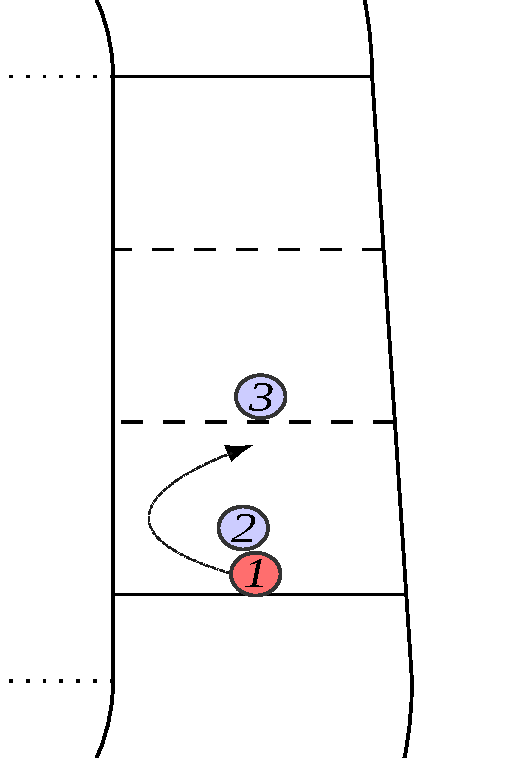
\includegraphics[scale=0.75,trim={0.5cm 1cm 0 3cm}, clip]{img/billy_goat/1}
{\centering \it Passing the first blocker. First blocker is only allowed a few feet of movement.} 
\end{centering}
\end{minipage}
\hfill
\hspace{0.15cm}
\begin{minipage}{0.28\textwidth}
\begin{centering}
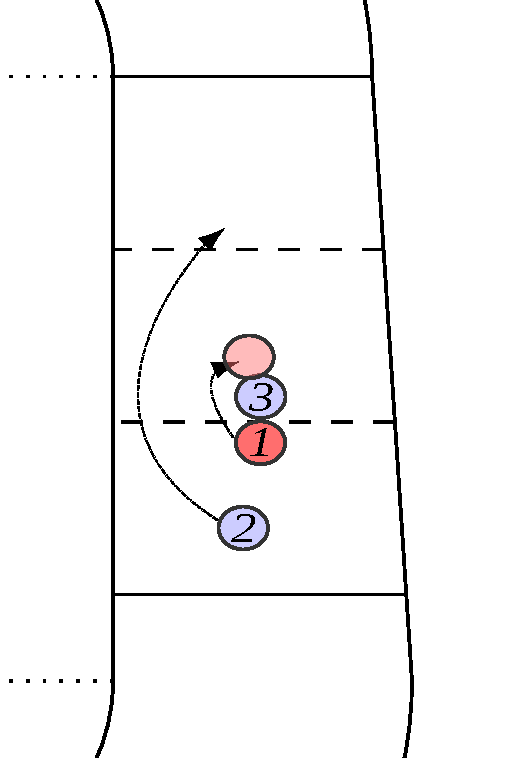
\includegraphics[scale=0.75,trim={0.5cm 1cm 0 3cm}, clip]{img/billy_goat/2}
{\centering \it Catching the second blocker as a goat. First blocker takes position.} 
\end{centering}
\end{minipage}
\hfill
\hspace{0.15cm}
\begin{minipage}{0.28\textwidth}
\begin{centering}
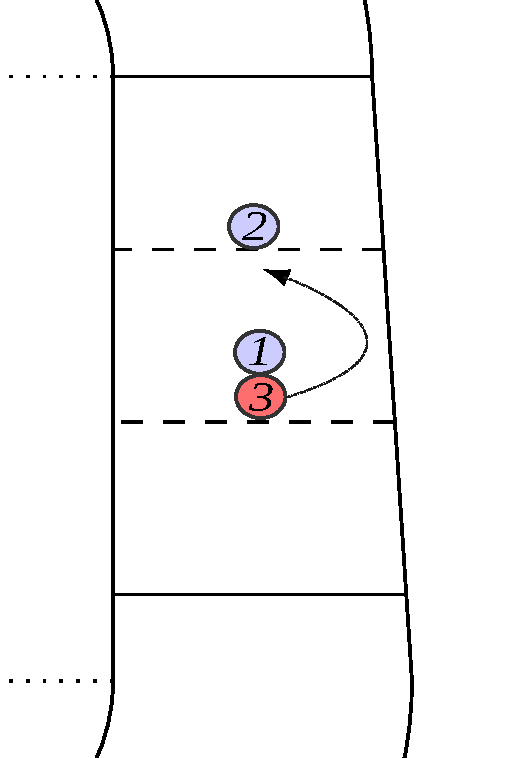
\includegraphics[scale=0.75,trim={0.5cm 1cm 0 3cm}, clip]{img/billy_goat/3}
{\centering \it Drill resets with skaters having rotated positions and with a new goat.} 
\end{centering}
\end{minipage}
\hfill





% TODO: Figure
